\documentclass[11pt]{article}

\usepackage[margin=1in]{geometry}
\usepackage{amsmath,amssymb,amsthm,mathtools}
\usepackage{bm}
\usepackage{enumitem}
\usepackage{hyperref}
\usepackage[dvipsnames]{xcolor}
\usepackage{tikz}
\usetikzlibrary{arrows.meta,calc,positioning,decorations.pathreplacing,patterns}
\usepackage{booktabs}
\usepackage{microtype}
\usepackage[T1]{fontenc}
\usepackage{lmodern}
\hypersetup{colorlinks=true, linkcolor=MidnightBlue, urlcolor=MidnightBlue, citecolor=MidnightBlue}

\newtheorem{definition}{Definition}
\newtheorem{problem}{Problem}
\newtheorem{remark}{Remark}
\newtheorem{assumption}{Assumption}
\newtheorem{theorem}{Theorem}
\newtheorem{proposition}{Proposition}

\title{\textbf{Magnetic Field--Supported Levitation and Control in a Bounded Domain}\\
\large Graduate Assignment}
\author{}
\date{}

\begin{document}
\maketitle

\begin{abstract}
This assignment studies whether a rigid spherical robot can be levitated, stabilized, and transported inside a cube whose six faces contain independently controlled electromagnetic boundary actuators. The document is written in a deliberately research-oriented style: students are asked to formalize the model, state assumptions precisely, derive equilibrium and stability conditions, and distinguish between an abstract force-field model and a physically realizable electromagnetic model. Particular emphasis is placed on force balance, local stabilizability, actuator limits, and the gap between idealized static levitation and what would be required for a real experimental implementation.
\end{abstract}

\section{Problem Overview}
We consider the problem of controlling the motion of a rigid spherical robot inside a bounded three-dimensional domain using externally generated electromagnetic fields. Specifically, a spherical robot is placed inside a cube whose six faces contain independently controllable electromagnetic actuators. These actuators generate a spatially varying field that produces forces and, in general, torques on the robot.

The primary objectives are:
\begin{enumerate}[label=\arabic*.]
    \item static levitation at arbitrary admissible points in the interior,
    \item stabilization under perturbations,
    \item controlled transport between points using feedback control.
\end{enumerate}

Students are asked to formalize the system, analyze its properties, and design appropriate control strategies.

\begin{figure}[t]
\centering
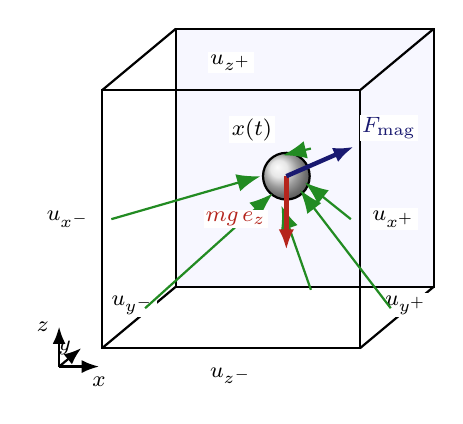
\begin{tikzpicture}[scale=0.78, every node/.style={font=\footnotesize}]
    % back face
    \coordinate (A) at (0,0);
    \coordinate (B) at (4.2,0);
    \coordinate (C) at (4.2,4.2);
    \coordinate (D) at (0,4.2);
    % front face offset
    \coordinate (E) at (1.2,1.0);
    \coordinate (F) at (5.4,1.0);
    \coordinate (G) at (5.4,5.2);
    \coordinate (H) at (1.2,5.2);

    \fill[blue!3] (E)--(F)--(G)--(H)--cycle;
    \draw[thick] (A)--(B)--(C)--(D)--cycle;
    \draw[thick] (E)--(F)--(G)--(H)--cycle;
    \draw[thick] (A)--(E) (B)--(F) (C)--(G) (D)--(H);

    % axes for orientation
    \draw[-{Latex[length=2.2mm]}, thick] ($(A)+(-0.7,-0.3)$) -- ++(0.65,0) node[below] {$x$};
    \draw[-{Latex[length=2.2mm]}, thick] ($(A)+(-0.7,-0.3)$) -- ++(0.36,0.3) node[left] {$y$};
    \draw[-{Latex[length=2.2mm]}, thick] ($(A)+(-0.7,-0.3)$) -- ++(0,0.65) node[left] {$z$};

    % Actuator labels
    \node[fill=white, inner sep=1pt] at ($(A)!0.5!(D)+(-0.55,0)$) {$u_{x^-}$};
    \node[fill=white, inner sep=1pt] at ($(B)!0.5!(C)+(0.55,0)$) {$u_{x^+}$};
    \node[fill=white, inner sep=1pt] at ($(A)!0.5!(B)+(0,-0.45)$) {$u_{z^-}$};
    \node[fill=white, inner sep=1pt] at ($(D)!0.5!(C)+(0,0.45)$) {$u_{z^+}$};
    \node[fill=white, inner sep=1pt] at ($(A)!0.5!(E)+(-0.1,0.2)$) {$u_{y^-}$};
    \node[fill=white, inner sep=1pt] at ($(B)!0.5!(F)+(0.15,0.2)$) {$u_{y^+}$};

    % ball
    \coordinate (P) at (3.0,2.8);
    \shade[ball color=gray!25] (P) circle (0.38);
    \draw[thick] (P) circle (0.38);
    \node[fill=white, inner sep=1pt] at ($(P)+(-0.56,0.76)$) {$x(t)$};

    % arrows from faces to ball
    \draw[-{Latex[length=3mm]}, thick, ForestGreen] ($(A)!0.5!(D)+(0.15,0)$) -- ($(P)+(-0.42,0)$);
    \draw[-{Latex[length=3mm]}, thick, ForestGreen] ($(B)!0.5!(C)+(-0.15,0)$) -- ($(P)+(0.30,-0.10)$);
    \draw[-{Latex[length=3mm]}, thick, ForestGreen] ($(A)!0.5!(E)+(0.1,0.15)$) -- ($(P)+(-0.22,-0.28)$);
    \draw[-{Latex[length=3mm]}, thick, ForestGreen] ($(B)!0.5!(F)+(-0.1,0.15)$) -- ($(P)+(0.22,-0.22)$);
    \draw[-{Latex[length=3mm]}, thick, ForestGreen] ($(A)!0.5!(B)+(1.3,0.95)$) -- ($(P)+(-0.08,-0.48)$);
    \draw[-{Latex[length=3mm]}, thick, ForestGreen] ($(D)!0.5!(C)+(1.3,-0.95)$) -- ($(P)+(-0.06,0.34)$);

    % gravity and resultant
    \draw[-{Latex[length=2.6mm]}, ultra thick, BrickRed] (P) -- ++(0,-1.2)
        node[pos=0.58, left=6pt, fill=white, inner sep=0.8pt] {$mg\,e_z$};
    \draw[-{Latex[length=2.6mm]}, ultra thick, MidnightBlue] (P) -- ++(1.1,0.48)
        node[pos=1, above right=2pt, fill=white, inner sep=0.8pt] {$F_{\mathrm{mag}}$};
\end{tikzpicture}
\caption{Cube-shaped actuator domain with six independently controlled boundary inputs. The sphere at position $x(t)$ is acted on by gravity and the net field-induced force generated by the six face actuators. In a physical implementation, the $u_{\cdot}$ variables should be interpreted as current, voltage, or another actuator command, not as literal ``magnetic charges.''}
\label{fig:cube_setup}
\end{figure}

\section{Assumptions and Conventions}

\subsection{Geometry and Admissible Configuration Region}
The physical cube is
\[
\Omega = [0,L]^3 \subset \mathbb{R}^3.
\]
The robot is a rigid sphere of radius $r>0$. Therefore, the robot center of mass cannot occupy the full set $\Omega$ without intersecting the boundary. The admissible center-of-mass region is instead
\[
\Omega_r := [r,L-r]^3.
\]
All equilibrium points, trajectories, and target points in Problems 1--5 are assumed to lie in $\operatorname{int}(\Omega_r)$ unless stated otherwise.

\subsection{Coordinates and Sign Convention}
We adopt a fixed inertial Cartesian frame with basis vectors $e_x,e_y,e_z$, where $e_z=(0,0,1)^\top$ points upward. Gravity therefore acts as the constant body force $-mg\,e_z$.

\subsection{Robot Model}
\begin{itemize}[leftmargin=1.5em]
    \item The robot is a rigid sphere with mass $m>0$ and radius $r>0$.
    \item Position: $x(t)\in\Omega_r$.
    \item Velocity: $v(t)=\dot{x}(t)$.
    \item For Problems 1--5, the assignment is \emph{translation-only}. Either the robot orientation is fixed by assumption, or the magnetic coupling law has been reduced to a purely translational surrogate. Rotational dynamics may be introduced only in the optional extensions.
\end{itemize}

\subsection{Regularity and Input Assumptions}
Unless a problem explicitly states otherwise, assume:
\begin{enumerate}[label=(A\arabic*), leftmargin=2.2em]
    \item The actuator input is a measurable function $u:[0,\infty)\to\mathbb{R}^6$ satisfying the amplitude constraints given below.
    \item The disturbance $d:[0,\infty)\to\mathbb{R}^3$ is measurable and essentially bounded whenever it is included.
    \item All force-basis functions $g_i:\Omega_r\to\mathbb{R}^3$ and field-basis functions $B_i:\Omega_r\to\mathbb{R}^3$ used by the student are at least $C^1$ on an open neighborhood of $\Omega_r$; if second derivatives are invoked, assume $C^2$ regularity.
    \item No passive damping, aerodynamic drag, viscous friction, or hidden stabilizing term is present unless it is explicitly added and declared.
\end{enumerate}

\subsection{Abstract Translational Dynamics}
The translation-only dynamics are modeled as
\[
 m\ddot{x}(t)=F_{\mathrm{mag}}\bigl(x(t),u(t)\bigr)-mg\,e_z+d(t),
\]
where:
\begin{itemize}[leftmargin=1.5em]
    \item $g>0$ is gravitational acceleration,
    \item $u(t)\in\mathbb{R}^6$ is the actuator input vector,
    \item $d(t)$ is a bounded disturbance term, included only when robustness is being analyzed.
\end{itemize}

A mathematically convenient control-affine surrogate is
\[
F_{\mathrm{mag}}(x,u)=\sum_{i=1}^6 u_i\,g_i(x),
\]
where $g_i(x)\in\mathbb{R}^3$ is the force contribution of actuator $i$ per unit input. Students may use this surrogate for analysis, but they should distinguish it clearly from the more restrictive field-based models below.

\subsection{Physically Consistent Electromagnetic Interpretation}
To ensure the assignment remains meaningful for an eventual laboratory implementation, students should distinguish the abstract force model above from a more physical actuator model.

A physically grounded quasi-static formulation is:
\[
B(x,u)=\sum_{i=1}^6 u_i\,B_i(x),
\]
where $B_i(x)\in\mathbb{R}^3$ is the magnetic field contribution of face $i$ per unit input. Two physically relevant robot models are then:
\begin{enumerate}[label=(\alph*), leftmargin=1.8em]
    \item \textbf{Controlled or permanent dipole model:} if the robot carries a magnetic dipole moment $\mu\in\mathbb{R}^3$, then
    \[
    F_{\mathrm{mag}}(x,u)=\nabla\!\bigl(\mu\cdot B(x,u)\bigr),
    \qquad
    \tau_{\mathrm{mag}}(x,u)=\mu\times B(x,u).
    \]
    Equivalently, one may write $F_{\mathrm{mag}}=(\mu\cdot\nabla)B$ when $\mu$ is treated as constant in space.

    \item \textbf{Induced-dipole model:} if the sphere is magnetically polarizable with scalar susceptibility encoded by an effective coefficient $\alpha>0$, then a common surrogate is
    \[
    F_{\mathrm{mag}}(x,u)=\frac{\alpha}{2}\nabla \|B(x,u)\|^2.
    \]
\end{enumerate}

\noindent In either case, \emph{the force depends on field gradients, not only on field magnitude}. This distinction is essential if the model is later to be compared with experiments.

\begin{remark}[Why this matters for real testing]
A purely abstract map $F_{\mathrm{mag}}(x,u)$ is useful for control-theoretic analysis and simulation. However, if the model is intended to represent real hardware, it must encode at least the following: actuator limits, the mapping from electrical inputs to magnetic field, the robot's magnetic coupling mechanism, and the resulting force and torque law. Otherwise, the simulation may stabilize a mathematically convenient but physically unrealizable force field.
\end{remark}

\begin{remark}[Earnshaw-type obstruction and why feedback matters]
Students should not assume that a static magnetostatic field can automatically provide stable free-space levitation. In ordinary source-free magnetostatic settings, classical Earnshaw-type obstructions rule out broad classes of open-loop stable equilibria. Accordingly, Problems 1--5 should be interpreted as asking students to distinguish carefully between three questions: existence of force-balance equilibria, local stabilization under active feedback or time-varying control, and physically special material regimes that may evade the classical obstruction.
\end{remark}

\subsection{Actuator Constraints}
Assume bounded inputs
\[
 u_i\in[u_{\min},u_{\max}], \qquad i=1,\dots,6.
\]
Students may also assume rate limits $|\dot u_i|\leq \rho_i$ if desired, but any such assumption must be stated explicitly.

\section{Definitions}

\begin{definition}[Equilibrium]
A point $x^\star\in\operatorname{int}(\Omega_r)$ is an equilibrium if there exists $u^\star\in [u_{\min},u_{\max}]^6$ such that
\[
F_{\mathrm{mag}}(x^\star,u^\star)=mg\,e_z.
\]
\end{definition}

\begin{definition}[Local Asymptotic Stability]
An equilibrium $(x^\star,u^\star)$ is locally asymptotically stable if, under a feedback law $u=\pi(x,v)$, trajectories initialized sufficiently near $(x^\star,0)$ remain near $(x^\star,0)$ and satisfy
\[
\lim_{t\to\infty} x(t)=x^\star,
\qquad
\lim_{t\to\infty} v(t)=0.
\]
\end{definition}

\begin{definition}[Reachability Between Equilibria]
Two equilibrium points $x_0^\star$ and $x_1^\star$ are reachable if there exists a control input $u(t)$ satisfying the actuator constraints such that the resulting trajectory remains in $\operatorname{int}(\Omega_r)$ for all intermediate times and transfers the system from the equilibrium at $x_0^\star$ to the equilibrium at $x_1^\star$.
\end{definition}

\begin{definition}[Stabilizing Controller]
A controller $u=\pi(x,v,x^\star)$ is stabilizing if
\[
\lim_{t\to\infty}x(t)=x^\star
\qquad\text{and}\qquad
\lim_{t\to\infty}v(t)=0.
\]
\end{definition}

\begin{figure}[t]
\centering
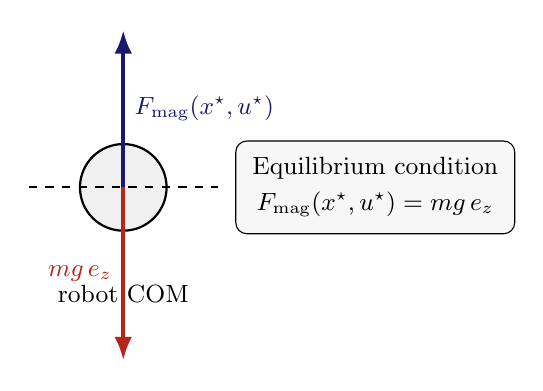
\begin{tikzpicture}[every node/.style={font=\small}]
    \coordinate (P) at (0,0);
    \draw[fill=gray!12, thick] (P) circle (0.55);
    \node at (0,-1.35) {robot COM};

    \draw[-{Latex[length=3mm]}, ultra thick, BrickRed] (P) -- ++(0,-2.2) node[midway,left] {$mg\,e_z$};
    \draw[-{Latex[length=3mm]}, ultra thick, MidnightBlue] (P) -- ++(0,2.0) node[midway,right] {$F_{\mathrm{mag}}(x^\star,u^\star)$};
    \draw[dashed, thick] (-1.2,0) -- (1.2,0);
    \node[draw, rounded corners, fill=gray!6, inner sep=6pt, align=center] at (3.2,0) {
    Equilibrium condition\\[2pt]
    $F_{\mathrm{mag}}(x^\star,u^\star)=mg\,e_z$
    };
\end{tikzpicture}
\caption{Static hover is a force-balance condition. In any physically meaningful model, the controller must choose an actuator command $u^\star$ such that the net field-induced force cancels gravity at the desired equilibrium point $x^\star$.}
\label{fig:force_balance}
\end{figure}

\begin{figure}[t]
\centering
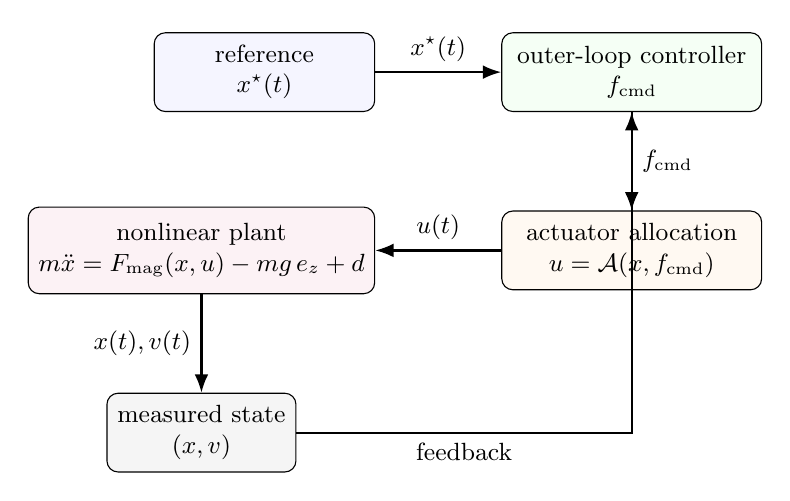
\begin{tikzpicture}[node distance=1.25cm and 1.6cm, every node/.style={font=\small, align=center}, >=Latex]
    \node[draw, rounded corners, minimum width=2.8cm, minimum height=1cm, fill=blue!4] (target) {reference\\ $x^{\star}(t)$};
    \node[draw, rounded corners, minimum width=3.3cm, minimum height=1cm, fill=green!4, right=of target] (controller) {outer-loop controller\\ $f_{\mathrm{cmd}}$};
    \node[draw, rounded corners, minimum width=3.3cm, minimum height=1cm, fill=orange!5, below=of controller] (allocator) {actuator allocation\\ $u=\mathcal{A}(x,f_{\mathrm{cmd}})$};
    \node[draw, rounded corners, minimum width=4.4cm, minimum height=1.1cm, fill=purple!5, left=of allocator] (plant) {nonlinear plant\\ $m\ddot x=F_{\mathrm{mag}}(x,u)-mg\,e_z+d$};
    \node[draw, rounded corners, minimum width=2.4cm, minimum height=1cm, fill=gray!8, below=of plant] (state) {measured state\\ $(x,v)$};

    \draw[->, thick] (target) -- node[above] {$x^\star(t)$} (controller);
    \draw[->, thick] (controller) -- node[right] {$f_{\mathrm{cmd}}$} (allocator);
    \draw[->, thick] (allocator) -- node[above] {$u(t)$} (plant);
    \draw[->, thick] (plant) -- node[left] {$x(t),v(t)$} (state);
    \draw[->, thick] (state) -| node[pos=0.25, below] {feedback} (controller);
\end{tikzpicture}
\caption{Recommended closed-loop interpretation. The cleanest formulation treats PID, LQR, or other feedback as generating a desired net force $f_{\mathrm{cmd}}$, followed by a separate actuator-allocation map $\mathcal{A}$ that respects actuator constraints and the chosen field model.}
\label{fig:control_loop}
\end{figure}

\section{Problems}

\begin{problem}[Equilibrium Existence]
Determine conditions under which
\[
\forall x^\star\in\operatorname{int}(\Omega_r),\qquad \exists u^\star
\]
such that $x^\star$ is an equilibrium point.

Questions to address:
\begin{itemize}[leftmargin=1.5em]
    \item What structural properties must the abstract force basis $\{g_i(x)\}$ or field basis $\{B_i(x)\}$ satisfy?
    \item Are six face actuators sufficient to generate arbitrary force directions throughout the entire admissible interior region, or does the answer depend on the chosen force law and geometry?
    \item How do actuator magnitude limits and geometric decay constrain the set of achievable equilibria?
\end{itemize}
\noindent Students should not assume that six scalar inputs imply arbitrary three-axis force authority: for example, induced-dipole forces arise from a gradient field and are therefore strongly constrained by the chosen magnetic model.
\end{problem}

\begin{problem}[Local Stability]
Linearize the dynamics about an equilibrium $(x^\star,0,u^\star)$ using $x=x^\star+\delta x$, $v=\delta v$, and $u=u^\star+\delta u$, and derive a local model of the form
\[
\delta \ddot x = A\,\delta x + B\,\delta u.
\]
Before applying stabilizability tests, pole placement, or LQR, rewrite this second-order model as a first-order state-space system in the augmented state $(\delta x,\delta v)$.

Tasks:
\begin{itemize}[leftmargin=1.5em]
    \item Determine conditions for stabilizability.
    \item Analyze whether PID control is sufficient in a local neighborhood.
    \item Compare PID with state-feedback or optimal linear control.
\end{itemize}
\noindent If PID is considered, state clearly whether it means three Cartesian loops that generate a desired net force, followed by actuator allocation, or a genuinely coupled MIMO dynamic compensator directly producing actuator commands.
\end{problem}

\begin{problem}[Controller Design]
Design a feedback law
\[
 u(t)=\pi\bigl(x(t),v(t),x^\star\bigr)
\]
such that:
\begin{itemize}[leftmargin=1.5em]
    \item convergence is achieved,
    \item control remains bounded,
    \item robustness to small disturbances and model mismatch is maintained.
\end{itemize}
Students may use PID, nonlinear feedback, or model-based control, provided the choice is justified and the controller architecture is specified precisely. Any solution that uses an outer-loop force command should also specify how actuator allocation is performed.
\end{problem}

\begin{problem}[Point-to-Point Transfer]
Given a desired trajectory $x^\star(t)$ joining two equilibrium points, construct a controller that:
\begin{itemize}[leftmargin=1.5em]
    \item tracks $x^\star(t)$,
    \item keeps velocity and acceleration bounded,
    \item converges to the final equilibrium.
\end{itemize}
Assume $x^\star(\cdot)$ is at least $C^2$ and lies in $\operatorname{int}(\Omega_r)$ for all times of interest. Discuss whether simple interpolation of the target is sufficient, or whether trajectory shaping and feedforward compensation are required to keep the reference dynamically admissible under the actuator bounds and field model.
\end{problem}

\begin{problem}[Fundamental Limitations]
Analyze the following:
\begin{enumerate}[label=\arabic*.]
    \item Can every point in the admissible center-of-mass region $\Omega_r$ be stabilized?
    \item How does field decay with distance alter controllability and the reachable equilibrium set?
    \item Under purely static field assumptions, can stable equilibrium exist without feedback? If not, explain the relevant obstruction.
\end{enumerate}
Provide proofs, counterexamples, or carefully reasoned arguments.
\end{problem}

\section{Theorem Targets}
A high-quality solution should aim to prove, disprove, or conditionally establish statements of the following type.

\begin{enumerate}[label=\textbf{T\arabic*:}, leftmargin=3em]
    \item \textbf{Equilibrium existence theorem.} Under explicit assumptions on the chosen actuator surrogate or field basis and actuator bounds, characterize a nonempty interior subset $\Omega_{\mathrm{eq}}\subseteq\Omega_r$ for which every $x^\star\in\Omega_{\mathrm{eq}}$ admits an equilibrium input $u^\star$.

    \item \textbf{Local stabilizability theorem.} Derive sufficient conditions on the geometry, operating point, and chosen force law under which the first-order linearization has a stabilizable pair $(A,B)$, and then prove that a local feedback law exists that renders the equilibrium locally asymptotically stable.

    \item \textbf{PID sufficiency theorem or counterexample.} After defining a precise PID architecture for the 3D system, preferably as an outer-loop desired-force controller together with an actuator-allocation map, state conditions under which it is sufficient for local stabilization, or construct a counterexample showing that PID fails without additional feedforward, allocation logic, or model-based compensation.

    \item \textbf{Tracking theorem.} For a sufficiently smooth target trajectory $x^\star(t)$ lying in an admissible operating region, derive conditions under which bounded tracking error can be guaranteed.

    \item \textbf{Limitation theorem.} Prove a statement showing that if the field model is restricted to static, source-free magnetostatic actuation with no active feedback and no special material effects, then globally stable free-space levitation is generically impossible or strongly restricted.
\end{enumerate}

\section{Extensions (Optional)}
Students may explore any of the following:
\begin{itemize}[leftmargin=1.5em]
    \item rotational dynamics,
    \[
    I\dot\omega = \tau_{\mathrm{mag}},
    \]
    \item hybrid control using external field actuation plus onboard thrusters,
    \item energy-based control and potential shaping,
    \item actuator bandwidth and rate constraints,
    \item simulation studies validating the proposed controller.
\end{itemize}

\section{Deliverables}
Each submission must include:
\begin{enumerate}[label=\arabic*.]
    \item formal derivations,
    \item clearly stated assumptions,
    \item controller design and justification,
    \item stability analysis,
    \item discussion of limitations,
    \item optional simulation results.
\end{enumerate}

\section{Expected Insights}
Strong solutions should recognize the following.
\begin{itemize}[leftmargin=1.5em]
    \item Levitation is a force-balance problem, not gravity cancellation.
    \item A physically meaningful model must specify how actuator inputs generate magnetic field and field gradients.
    \item Static force balance does not by itself imply open-loop stability; Earnshaw-type limitations matter.
    \item Local stabilization typically requires active feedback.
    \item The system is nonlinear even before rotational dynamics are included.
    \item PID may be useful locally but may fail globally or under severe actuator limits.
    \item Field decay, input saturation, and geometric constraints strongly restrict what can be achieved in practice.
\end{itemize}

\section{Practical Note on Modeling Fidelity}
If this problem is later tested in simulation or hardware, the following hierarchy is recommended.
\begin{enumerate}[label=\arabic*.]
    \item Begin with the abstract control-affine model $F_{\mathrm{mag}}(x,u)$, optionally augmented later by an explicitly defined damping or drag term, for theorem development and controller prototyping.
    \item Upgrade to a quasi-static field model $B(x,u)=\sum_i u_i B_i(x)$ to preserve physical interpretability.
    \item Include the appropriate force law for the robot's actual magnetic coupling mechanism: permanent dipole, induced dipole, superconducting element, or other design.
    \item Add actuator limits, bandwidth limits, and measurement noise before claiming that a controller is viable in real hardware.
\end{enumerate}
This structure preserves mathematical tractability while keeping the assignment aligned with forces and equations that could, in principle, be tested experimentally.

\section{Summary}
This assignment studies whether a programmable electromagnetic boundary field can function as a controllable three-dimensional virtual-gravity system and what control laws are required to achieve stable levitation and motion. The analysis is intentionally split between an abstract nonlinear control problem and a physically realizable electromagnetic interpretation so that successful solutions remain useful both mathematically and experimentally.

\end{document}
